\begin{appendices}

  \section{Enunciado del trabajo práctico}

    \subsection{Introducción}

      Consideremos la sección horizontal de un horno de acero cilíndrico, como en la Figura \ref{fig:seccionHorno}. El sector A es la pared del horno, y el sector B es el horno propiamente dicho, en el cual se funde el acero a temperaturas elevadas. Tanto el borde externo como el borde interno de la pared forman círculos. Suponemos que la temperatura del acero dentro del horno (o sea, dentro de B) es constante e igual a 1500{\degree}C.
      Tenemos sensores ubicados en la parte externa del horno para medir la temperatura de la pared externa del mismo, que habitualmente se encuentra entre 50{\degree}C y 200{\degree}C. El problema que debemos resolver consiste en estimar la isoterma de 500{\degree}C dentro de la pared del horno, para estimar la resistencia de la misma. Si esta isoterma está demasiado cerca de la pared externa del horno, existe peligro de que la estructura externa de la pared colapse.

      \begin{figure}[h]
        \centering
        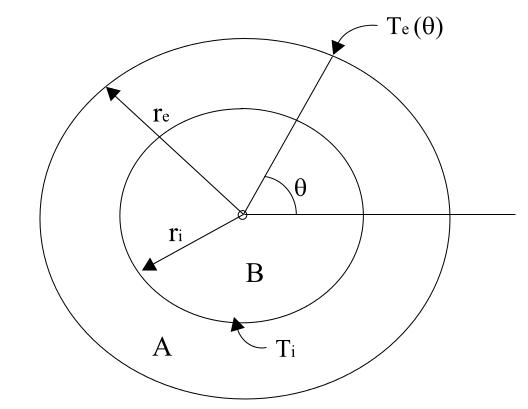
\includegraphics[width=10cm]{seccionHorno.jpg}
        \caption{Sección circular del horno.}
        \label{fig:seccionHorno}
      \end{figure}

      El objetivo del trabajo práctico es implementar un programa que calcule la isoterma solicitada, conociendo las dimensiones del horno y las mediciones de temperatura en la pared exterior.

    \subsection{El Modelo}

      Sea $r_e \in \mathbb{R}$ el radio exterior de la pared y sea $r_i \in \mathbb{R}$ el radio interior de la pared. Llamemos $T(r, \theta)$ a la temperatura en el punto dado por las coordenadas polares $(r, \theta)$, siendo $r$ el radio y $\theta$ el ángulo polar de dicho punto. En el estado estacionario, esta temperatura satisface la ecuación del calor:

      \begin{equation} \label{eq:en1}
        \frac{\partial^2 T(r, \theta)}{\partial r^2} + \frac{1}{r} \frac{\partial T(r, \theta)}{\partial r} + \frac{1}{r^2} \frac{\partial^2 T(r, \theta)}{\partial \theta^2} = 0
      \end{equation}

      Si llamamos $T_i \in \mathbb{R}$ a la temperatura en el interior del horno (sector B) y $T_e : [0, 2\pi] \to \mathbb{R}$ a la función de temperatura en el borde exterior del horno (de modo tal que el punto $(r_e, \theta)$ tiene temperatura $T_e(\theta)$), entonces tenemos que

      \begin{equation} \label{eq:en2}
        T(r, \theta) = T_i \text{ para todo punto } (r, \theta) \text{ con } r \leq r_i
      \end{equation}

      \begin{equation} \label{eq:en3}
        T(r_e, \theta) = T_e(\theta) \text{ para todo punto } (r_e, \theta)
      \end{equation}

      El problema en derivadas parciales dado por la primera ecuación con las condiciones de contorno presentadas recientemente, permite encontrar la función $T$ de temperatura en el interior del horno (sector A), en función de los datos mencionados en esta sección.

      Para resolver este problema computacionalmente, discretizamos el dominio del problema (el sector A) en coordenadas polares. Consideramos una partición $0 = \theta_0 < \theta_1 < ... < \theta_n = 2\pi$ en $n$ ángulos discretos con $\theta_k - \theta_{k-1} = \Delta \theta$ para $k = 1, \dots n$, y una partición $r_i = r_0 < r_1 < ... < r_m = r_e$ en $m + 1$ radios discretos con $r_j - r_{j-1} = \Delta r$ para $j = 1, \dots m$.

      El problema ahora consiste en determinar el valor de la función $T$ en los puntos de la discretización $(r_j, \theta_k)$ que se encuentren dentro del sector A. Llamemos $t_{jk} = T(r_j , \theta_k)$ al valor (desconocido) de la función $T$ en el punto $(r_j, \theta_k)$.

      Para encontrar estos valores, transformamos la ecuación (\ref{eq:en1}) en un conjunto de ecuaciones lineales sobre las incógnitas $t_{jk}$, evaluando (\ref{eq:en1}) en todos los puntos de la discretización que se encuentren dentro del sector A. Al hacer esta evaluación, aproximamos las derivadas parciales de $T$ en (\ref{eq:en1}) por medio de las siguientes fórmulas de diferencias finitas:

      \begin{equation} \label{eq:en4}
        \frac{\partial^2 T(r, \theta)}{\partial r^2}(r_j, \theta_k) \cong \frac{t_{j-1,k} - 2 t_{jk} + t_{j+1,k}}{(\Delta r)^2}
      \end{equation}

      \begin{equation} \label{eq:en5}
        \frac{\partial T(r, \theta)}{\partial r}(r_j, \theta_k) \cong \frac{t_{j,k} - t_{j-1,k}}{\Delta r}
      \end{equation}

      \begin{equation} \label{eq:en6}
        \frac{\partial^2 T(r, \theta)}{\partial \theta^2}(r_j, \theta_k) \cong \frac{t_{j,k-1} - 2 t_{jk} + t_{j,k+1}}{(\Delta \theta)^2}
      \end{equation}

      Es importante notar que los valores de las incógnitas son conocidos para los puntos que se encuentran sobre el borde exterior de la pared, y para los puntos que se encuentren dentro del sector B. Al realizar este procedimiento, obtenemos un sistema de ecuaciones lineales que modela el problema discretizado. La resolución de este sistema permite obtener una aproximación de los valores de la función $T$ en los puntos de la discretización.

    \subsection{Enunciado}
      Se debe implementar un programa en \texttt{C} o \texttt{C++} que tome como entrada los parámetros del problema ($r_i$, $r_e$, $m + 1$, $n$, valor de la isoterma buscada, $T_i$, $T_e(\theta)$) que calcule la temperatura dentro de la pared del horno utilizando el modelo propuesto en la sección anterior y que encuentre la isoterma buscada en función del resultado obtenido del sistema de ecuaciones. El método para determinar la posición de la isoterma queda a libre elección de cada grupo y debe ser explicado en detalle en el informe.

      El programa debe formular el sistema obtenido a partir de las ecuaciones (\ref{eq:en1})-(\ref{eq:en6}) y considerar dos métodos posibles para su resolución: mediante el algoritmo clásico de Eliminación Gaussiana y la Factorización LU. Finalmente, el programa escribirá en un archivo la solución obtenida con el formato especificado en la siguiente sección.

      Como ya se ha visto en la materia, no es posible aplicar los métodos propuestos para la resolución a cualquier sistema de ecuaciones. Sin embargo, la matriz del sistema considerado en el presente trabajo cumple con ser diagonal dominante (no estricto) y que, ordenando las variables y ecuaciones convenientemente, es posible armar un sistema de ecuaciones cuya matriz posee la propiedad de ser \emph{banda}. Luego, se pide demostrar (o al menos dar un esquema de la demostración) el siguiente resultado e incluirlo en el informe:

      \begin{prop}
        Sea $A \in \mathbb{R}^{n \times n}$ la matriz obtenida para el sistema definido por (\ref{eq:en1})-(\ref{eq:en6}). Demostrar que es posible aplicar Eliminación Gaussiana sin pivoteo.\footnote{Sugerencia: Notar que la matriz es diagonal dominante (no estrictamente) y analizar qué sucede al aplicar un paso de Eliminación Gaussiana con los elementos de una fila.}
      \end{prop}

      La solución del sistema de ecuaciones permitirá saber la temperatura en los puntos de la discretización. Sin embargo, nuestro interés es calcular la isoterma 500, para poder determinar si la estructura se encuentra en peligro. Luego, se pide lo siguiente:

      \begin{itemize}
        \item Dada la solución del sistema de ecuaciones, proponer una forma de estimar en cada ángulo de la discretización la posición de la isoterma 500.
        \item En función de la aproximación de la isoterma, proponer una forma (o medida) a utilizar para evaluar la peligrosidad de la estructura en función de la distancia a la pared externa del horno.
      \end{itemize}

      En función de la experimentación, se busca realizar dos estudios complementarios: por un lado, analizar cómo se comporta el sistema y, por otro, cuáles son los requerimientos computacionales de los métodos. Se pide como mínimo realizar los siguientes experimentos:

      \begin{enumerate}
        \item Comportamiento del sistema.
          \begin{itemize}
            \item Considerar al menos dos instancias de prueba, generando distintas discretizaciones para cada una de ellas y comparando la ubicación de la isoterma buscada respecto de la pared externa del horno. Se sugiere presentar gráficos de temperatura o curvas de nivel para los mismos, ya sea utilizando las herramientas provistas por la cátedra o implementando sus propias herramientas de graficación.
            \item Estudiar la proximidad de la isoterma buscada respecto de la pared exterior del horno en función de distintas granularidades de discretización y las condiciones de borde.
          \end{itemize}

        \item Evaluación de los métodos.
          \begin{itemize}
            \item Analizar el tiempo de cómputo requerido para obtener la solución del sistema en función de la granularidad de la discretización. Se sugiere presentar los resultados mediante gráficos de tiempo de cómputo en función de alguna de las variables del problema.
            \item Considerar un escenario similar al propuesto en el experimento 1. pero donde las condiciones de borde (i.e., $T_i$ y $T_e(\theta)$) cambian en distintos instantes de tiempo. En este caso, buscamos obtener la secuencia de estados de la temperatura en la pared del horno, y la respectiva ubicación de la isoterma especificada. Para ello, se considera una secuencia de $ninst$ vectores con las condiciones de borde, y las temperaturas en cada estado es la solución del correspondiente sistema de ecuaciones. Se pide formular al menos un experimento de este tipo, aplicar los métodos de resolución propuestos de forma conveniente y compararlos en términos de tiempo total de cómputo requerido para distintos valores de $ninst$.
          \end{itemize}
      \end{enumerate}

      De manera opcional, aquellos grupos que quieran ir un poco más allá pueden considerar trabajar y desarrollar alguno(s) de los siguientes puntos extra:
      \begin{enumerate}
        \item Notar que el sistema resultante tiene estructura \emph{banda}. Proponer una estructura para aprovechar este hecho en términos de la \emph{complejidad espacial} y como se adaptarían los algoritmos de Eliminación Gaussiana y Factorización LU para reducir la cantidad de operaciones a realizar.
        \item Implementar dicha estructura y las adaptaciones necesarias para el algoritmo de Eliminación Gaussiana.
        \item Implementar dicha estructura y las adaptaciones necesarias para el algoritmo de Factorización LU.
      \end{enumerate}

      Finalmente, se deberá presentar un informe que incluya una descripción detallada de los métodos implementados y las decisiones tomadas, el método propuesto para el cálculo de la isoterma buscada y los experimentos realizados, junto con el correspondiente análisis y siguiendo las pautas definidas en el archivo \texttt{pautas.pdf}.

    \subsection{Programa y formato de archivos}
      Se deberán entregar los archivos fuentes que contengan la resolución del trabajo práctico. El ejecutable tomará tres parámetros por línea de comando, que serán el archivo de entrada, el archivo de salida, y el método a ejectutar (0 Eliminación Gaussiana, 1 LU).

      El archivo de entrada tendrá la siguiente estructura:
      \begin{itemize}
        \item La primera línea contendrá los valores $r_i$, $r_e$, $m + 1$, n, iso, $ninst$, donde $iso$ representa el valor de la isoterma buscada y $ninst$ es la cantidad de instancias del problema a resolver para los parámetros dados.
        \item A continuación, el archivo contendrá $ninst$ líneas, cada una de ellas con $2 n$ valores, los primeros $n$ indicando los valores de la temperatura en la pared interna, i.e., $T_i(\theta_0), T_i(\theta_1), \dots, T_i(\theta_n-1)$, seguidos de $n$ valores de la temperatura en la pared externa, i.e., $T_e(\theta_0), T_e(\theta_1), \dots, T_e(\theta_n-1)$.
      \end{itemize}

      El archivo de salida obligatorio tendrá el vector solución del sistema reportando una componente del mismo por línea. En caso de $ninst > 1$, los vectores serán reportados uno debajo del otro.

      Junto con el presente enunciado, se adjunta una serie de scripts hechos en \texttt{python} y un conjunto instancias de test que deberán ser utilizados para la compilación y un testeo básico de la implementación. Se recomienda leer el archivo \texttt{README.txt} con el detalle sobre su utilización.

    \subsection{Fechas de entrega}
      \begin{itemize}
        \item \emph{Formato Electrónico}: Jueves 3 de Septiembre de 2015, hasta las 23:59 hs, enviando el trabajo (informe + código) a la dirección \texttt{metnum.lab@gmail.com}. El subject del email debe comenzar con el texto \texttt{[TP1]} seguido de la lista de apellidos de los integrantes del grupo.
        \item \emph{Formato físico}: Viernes 4 de Septiembre de 2015, de 17:30 a 18:00 hs.
      \end{itemize}

      \strong{Importante}: El horario es estricto. Los correos recibidos después de la hora indicada serán considerados re-entrega. Los grupos deben ser de 3 o 4 personas, sin excepción. Es indispensable que los trabajos pasen satisfactoriamente los casos de test provistos por la cátedra.

  \newpage
  \section{Código fuente}

    {\color{Gray} En el apéndice B se incluirán los códigos fuente de las funciones relevantes desde el punto de vista numérico.

    Podemos incluir archivos de código:
    \lstinputlisting[language=C++, firstline=0, lastline=18, style=customcpp]{../src/altohorno.cpp}}

\end{appendices}
